\documentclass{article}

% Margin definition.
\usepackage[a4paper,total={6.8in, 8.5in}]{geometry}
\usepackage{parskip}
\usepackage[bottom]{footmisc}
% Images.
\usepackage{graphicx}
\usepackage[export]{adjustbox}
\usepackage{float}
% Table
\usepackage{array}
\usepackage[toc,page]{appendix}
% Links.
\usepackage[T1,hyphens]{url}
\usepackage[hidelinks, bookmarks=true]{hyperref}
% Encoding.
\usepackage[utf8]{inputenc}
% Helvetic font.
\usepackage[scaled]{helvet}
\renewcommand\familydefault{\sfdefault} 
% Header for ua logo.
\usepackage{fancyhdr}
% Dots in index.
\usepackage[titles]{tocloft}
\renewcommand{\cftsubsubsecleader}{\Large\cftdotfill{0}}
\renewcommand{\cftsubsecleader}{\Large\cftdotfill{0}}
\renewcommand{\cftsecleader}{\Large\cftdotfill{0}}
\renewcommand{\cftsecfont}{\large\bfseries\scshape}
\renewcommand{\cftsubsecfont}{\scshape}
\renewcommand{\cftsubsubsecfont}{\small\scshape}
\addtolength{\cftsecnumwidth}{5pt}
\renewcommand*{\HyperDestNameFilter}[1]{\jobname-#1}
% Dot after number in (sub)sections and in toc.
\renewcommand{\cftsecaftersnum}{.}
\renewcommand{\cftsubsecaftersnum}{}
\usepackage[letterspace=45]{microtype}
\newcommand*{\fullref}[1]{\hyperref[{#1}]{\autoref*{#1} \nameref*{#1} \urlref*{#1}}}
% Header with ua logo definition. 
\pagestyle{fancy}
\fancyhf{}
\chead{
    
\includegraphics[height=0.5in]{./img/header_ua.png}
}
\setlength\headheight{45pt}
% Footer with page number.
\rfoot{Página \thepage}
\renewcommand{\footrulewidth}{0.4pt}
% Rename table of contents title to "Index"
\renewcommand{\contentsname}{\normalsize Indice \vspace{0.6cm}}

% for code
\usepackage{listings}
\usepackage{xcolor}

\definecolor{codegreen}{rgb}{0,0.6,0}
\definecolor{codegray}{rgb}{0.5,0.5,0.5}
\definecolor{codepurple}{rgb}{0.58,0,0.82}
\definecolor{backcolour}{rgb}{0.95,0.95,0.92}

\lstdefinestyle{mystyle}{
    backgroundcolor=\color{backcolour},   
    commentstyle=\color{codegreen},
    keywordstyle=\color{magenta},
    numberstyle=\tiny\color{codegray},
    stringstyle=\color{codepurple},
    basicstyle=\ttfamily\footnotesize,
    breakatwhitespace=false,         
    breaklines=true,                 
    captionpos=b,                    
    keepspaces=true,                 
    numbers=left,                    
    numbersep=5pt,                  
    showspaces=false,                
    showstringspaces=false,
    showtabs=false,                  
    tabsize=2
}

\lstset{style=mystyle}


% for the references
\usepackage[nottoc,numbib]{tocbibind}

% section on new page, except the index one
\usepackage{etoolbox}
\pretocmd{\section}{%
  \ifnum\value{section}=0 \else\clearpage\fi
}{}{}


%encoding
%--------------------------------------
\usepackage[T1]{fontenc}
\usepackage[utf8]{inputenc}
%--------------------------------------

%Portuguese-specific commands
%--------------------------------------
\usepackage[portuguese]{babel}
%--------------------------------------

%Hyphenation rules
%--------------------------------------
\usepackage{hyphenat}
\hyphenation{mate-mática recu-perar}
%--------------------------------------

\usepackage{mathtools}
\usepackage{makecell}

\begin{document}

\title{\vspace{-0.9cm}
       \large\raggedright\textbf{} \\ 
       \vspace{0.5cm}
       \normalsize
       \raggedright\textbf{Titulo: \hspace{1.1cm} Evolução do número de utilizadores do Signal em relação à concorrência} \\ \vspace{0.4cm}
       \raggedright\textbf{Autor: \hspace{1.13cm} Pedro Miguel Nicolau Escaleira} \\ \vspace{0.4cm}
       \raggedright\textbf{Date: \hspace{1.3cm} 12/06/2020} \\}
\author{}
\date{}

\maketitle
\thispagestyle{fancy}

\vspace{-1.4cm}

\tableofcontents

\newpage

\fontsize{10pt}{13pt}
\selectfont
\lsstyle

\section{Introdução}

O \textit{Signal} é uma aplicação de \textit{messaging} multi-plataforma que, tal como outras opções existentes no mercado, como o \textit{WhatsApp} ou o \textit{Facebook Messenger}, permite aos seus utilizadores enviar e receber mensagens de texto, voz ou multimédia \textit{online}. O foco principal deste serviço é permitir que os seus utilizadores comuniquem entre si de forma totalmente segura e privada, oferecendo \textit{End-to-end encryption}.

O trabalho apresentado neste relatório enquadra-se no seguimento do estudo do funcionamento da aplicação \textit{Signal} apresentada em \cite{past_report}.

Neste documento irá ser analisada e interpretada uma possível evolução do número de utilizadores deste serviço em relação aos seus principais concorrentes no mercado. Como ponto de partida, irá ser analisado o crescimento que cada uma destas aplicações teve no passado e, com este conhecimento em atenção, irá ser apresentado um modelo que tente prever o futuro. 

% história da aplicação
% mercado no passado e presente (do signal e concorrência)

\section{Contexto histórico}

\subsection{Origem}     % ver o titulo
Ao contrário de outras aplicações do mesmo estilo, como o \textit{WhatsApp}, que foram criadas sob a alçada de grandes empresas, com um grande financiamento desde o inicio, o \textit{Signal} foi criado como um projeto \textit{open-source} pelo investigador de cibersegurança \textbf{Moxie Marlinspike}. A primeira versão foi lançada em 2014. Desde o inicio que o propósito principal da aplicação é permitir aos seus utilizadores privacidade total quando comunicam usando o serviço, usando para isso um protocolo desenvolvido especialmente para o \textit{Signal}, o \textit{Signal Protocol}, que concede encriptação ponto a ponto ás comunicações feitas.

Apesar do \textit{Signal Protocol} ter sido criado para ser utilizado pelo \textit{Signal}, houve outras aplicações de outras empresas com interesse em usar este protocolo para permitir comunicações seguras sob a sua alçada:

\begin{itemize}
   \item \textbf{\textit{Facebook Messenger}} - Integrada em 2016 o protocolo como uma \textit{feature} adicional para possíveis comunicações mais seguras.
   
   \item \textbf{\textit{Skype}} - Integrada em 2018, como uma nova \textit{feature} em \textit{chats} do tipo \textit{Private Conversations}.
   
   \item \textbf{\textit{WhatsApp}} - Integrada em 2016, sendo que a utilização \textit{default} da aplicação utiliza o protocolo para todas as comunicações. 
\end{itemize}

Sendo que o \textit{Signal} pertence a uma organização sem fins lucrativos (atualmente, \textit{Signal Foundation}), não possui um plano financeiro estável, sobrevivendo de doações feitas por utilizadores e apoiantes da filosofia do serviço. Em 2018, o co-fundador do \textit{WhatsApp}, Brian Acton, doou 50 milhões de dólares à \textit{Signal Foundation} como uma forma de propulsionar o acesso facilitado à possibilidade de realizar comunicações seguras a qualquer cidadão. \cite{history}


\subsection{Presença no mercado}

\section{Modelo de simulação}
\label{sec:model}

\subsection{Ferramenta utilizada}
A ferramenta escolhida para criar e executar o sistema dinâmico usado para simular o crescimento do número de utilizadores foi o \textit{Vensim}. De forma a aprender a usar esta ferramenta, foram seguidas as instruções apresentadas em \cite{vensim_youtube} e \cite{teacher_vensim}.

\subsection{Modelo criado}
O modelo criado em \textit{Vensim} está apresentado na figura \ref{model:vensim_model}. Este apresenta algumas similaridades com o segundo modelo apresentado no documento \cite{teacher_vensim} já que, sendo que a utilização duma aplicação depende da qualidade das \textit{features} que apresenta, alguns conceitos foram adaptados para este caso de estudo.

\begin{figure}[H]
   \begin{center}
       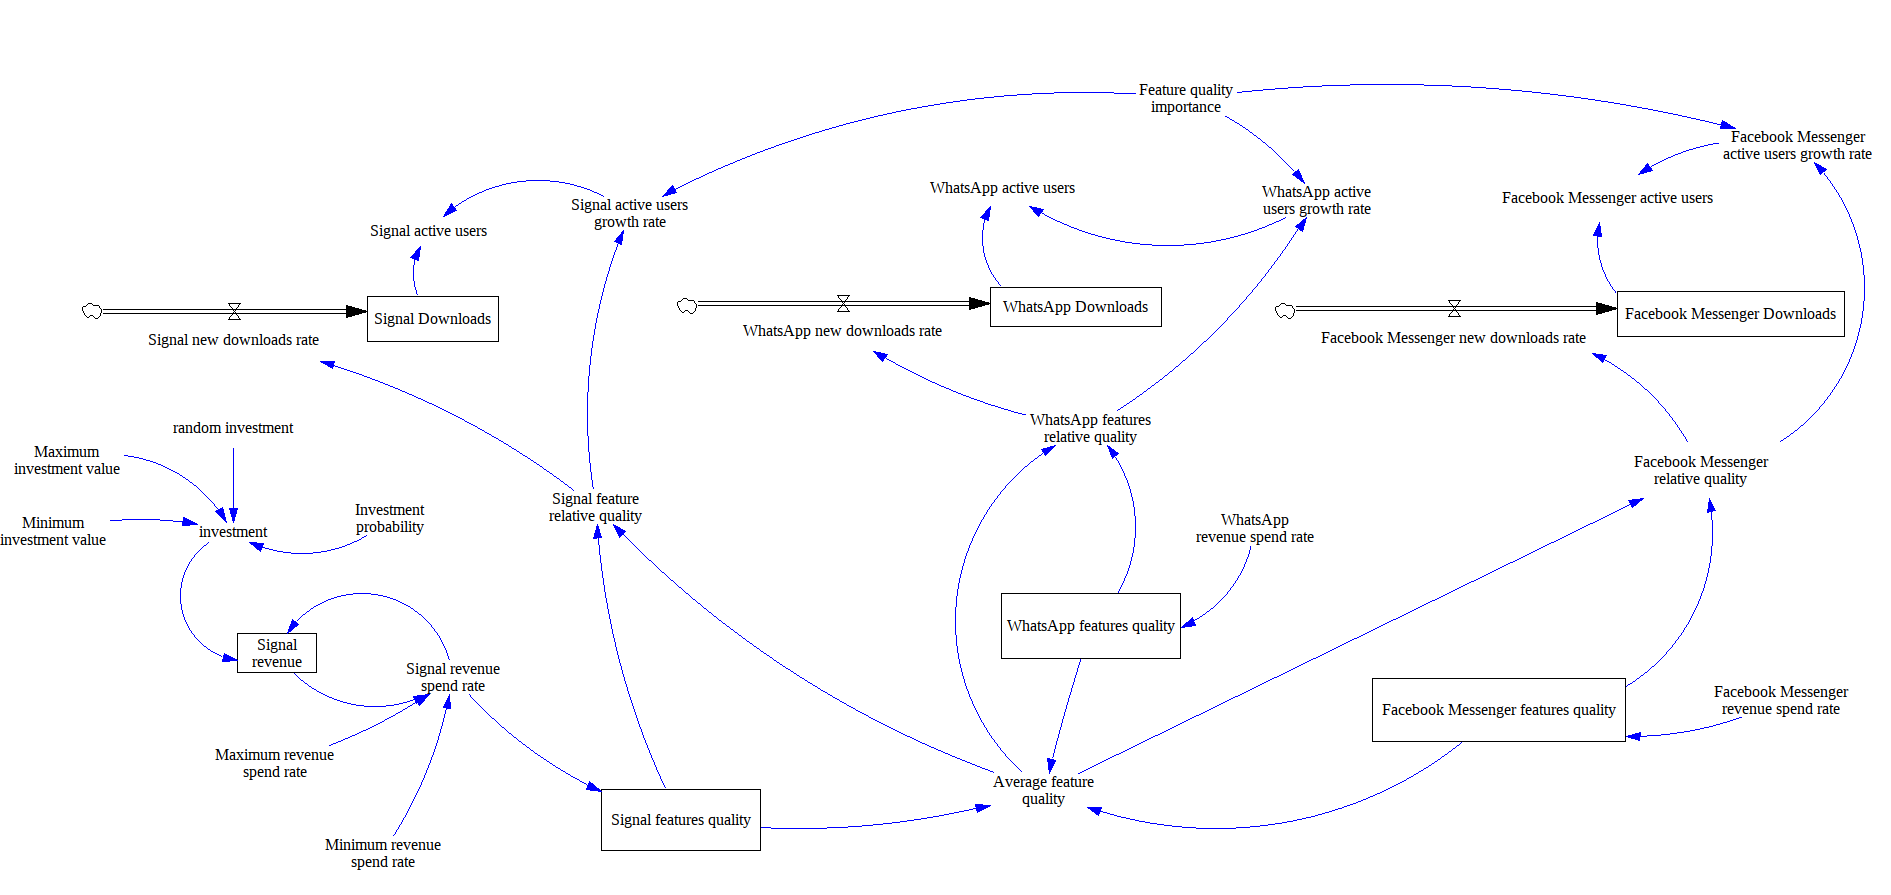
\includegraphics[width=17cm]{img/vensim_model.png}
       \caption{Modelo dinâmico criado em \textit{Vensim}.}
       \label{model:vensim_model}
   \end{center}
\end{figure}

Para a construção deste modelo, foram tidos alguns comportamentos verificados no passado do crescimento destes serviços em conta (ter em atenção que a unidade de tempo tida em conta neste modelo foi o \textit{Mês}):

\begin{itemize}
   \item Possíveis investimentos à \textit{Signal foundation}. Como explicado pelo fundador do \textit{Signal}, Moxie Marlinspike, o grande investimento de 50 milhões de dólares feito em 2018 pelo co-fundador do \textit{WhatsApp} foi um passo importante para aumentar o número de trabalhadores de 3 para atualmente 20. Com mais trabalhadores, foi possível criar novas \textit{features} já suportadas por outras aplicações concorrentes, como reagir a mensagens com \textit{emojis} (tal como no \textit{Facebook Messenger}) ou o envio de \textit{stickers}, sem nunca comprometer a segurança do serviço \cite{wired_signal}. Sendo assim, neste modelo foi tida em conta uma probabilidade de ocorrer um grande investimento como este. A seguinte equação demonstra como foi calculada a probabilidade usada no modelo:
   
   \begin{equation}
      \begin{split}
         P(\textit{investimento num dado mês}) & = \frac{1}{(\textit{número de anos até ocorrer o primeiro investimento})*12} \\
         & = \frac{1}{(2018-2014)*12} \\
         & = \frac{1}{48}
      \end{split}
  \end{equation}

  \item Relação entre número de \textit{downloads} e número de utilizadores ativos mensais. Para isso, foi feito o calculo apresentado pela equação \ref{calc:rel} tendo-se em conta os dados do \textit{WhatsApp} e do \textit{Facebook Messenger}, tendo-se obtido nos dois casos uma relação de 28\% de utilizadores ativos em relação ao número de \textit{downloads} feitos no \textit{Google Play}.
  
  \begin{equation}
      \label{calc:rel}
      \begin{split}
         Relacao = \frac{\textit{número de utilizadores ativos mensalmente}}{\textit{número total de downloads}}
      \end{split}
   \end{equation}

   Com isso em conta, foi executado o modelo criado múltiplas vezes com vários valores da variável \textit{Feature quality importance}, até aos valores iniciais das variáveis \textit{WhatsApp active users growth rate} e \textit{Facebook Messenger active users growth rate} apresentarem um valor apróximado a 0.28, de forma a possuir um modelo cujas condições inicias fossem parecidas às reais.

   \item Gastos mensais de cada um dos serviços. No caso do \textit{Signal}, os gastos mensais foram calculados tendo em conta os investimentos e a receita total que a \textit{Signal foundation} teve até ao momento. Nos outros dois serviços, foi tido em conta que são serviços geridos por grandes empresas, possuindo gastos bem definidos ao longo do tempo. Para além disso, no caso destas duas aplicações, foi tida em conta o investimento apresentado em \cite{whatsapp_craft} e foi feita uma estimativa dos gastos mensais desde o lançamento da aplicação até ao momento de acordo com esse investimento.
   
   \item Valores iniciais de \textit{download rate} e do número de \textit{downloads}. Quanto à \textit{download rate} foi tido em conta o número de \textit{downloads} diários que se verificavam à data de criação do modelo no \textit{Google Play}, multiplicados por 30 para ter o valor médio mensal. No caso do número de \textit{downloads} iniciais, foi usado o número de \textit{downloads} que cada uma das aplicações possuía à data da criação do modelo no \textit{Google Play}. Estes valores foram já apresentados neste documento na secção \ref{sec:market_presence}.
   
   \item Valor inicial do investimento tido no \textit{Signal}. O valor inicial de rendimento to \textit{Signal} é de 50 milhões de dólares dado investimento feito em 2018 pelo co-fundador do \textit{WhatsApp}.
\end{itemize}

A tabela \ref{tab:variables} ilustra os valores ou equações que cada variável possui no modelo final.

\begin{table}[h]

   \centering
   \begin{adjustbox}{width=1\textwidth}
   \begin{tabular}{|l|l|l|l|l|}
   \hline
   \textbf{Variável} & \textbf{Equação/valor} & \textbf{Unidades} & \makecell{\textbf{Valor} \\ \textbf{máximo}} & \makecell{\textbf{Valor} \\ \textbf{mínimo}} \\
   \hline
   INITIAL TIME & \textit{0} & \textit{Month} &  &  \\\hline
   FINAL TIME & \textit{120} & \textit{Month} &  &  \\\hline
   Average feature quality & \makecell[l]{\textit{(Facebook Messenger features quality + Signal features quality +} \\ \textit{WhatsApp features quality)/3}} & \textit{quality} &  &  \\\hline
   Facebook Messenger active users & \textit{Downloads*Facebook Messenger active users growth rate} & \textit{people}  &  &  \\\hline
   Facebook Messenger active users growth rate & \textit{Feature quality importance*Facebook Messenger relative quality} &  &  &  \\\hline
   Facebook Messenger Downloads & \textit{INTEG (Facebook Messenger new downloads rate, 4.52277e+09)} & \textit{people} &  &  \\\hline
   Facebook Messenger features quality & \textit{INTEG (Facebook Messenger revenue spend rate*20, 100)} & \textit{quality} &  &  \\\hline
   Facebook Messenger new downloads rate & \textit{4.56322e+07*Facebook Messenger relative quality} & \textit{people/Month} & 0 &  \\\hline
   Facebook Messenger relative quality & \textit{Facebook Messenger features quality/Average feature quality} &  &  &  \\\hline
   Facebook Messenger revenue spend rate & \textit{0.4} & \textit{million dollars/Month} & 0 & 1 \\\hline
   Feature quality importance & \textit{0.27} &  &  &  \\\hline
   investment & \makecell[l]{\textit{IF THEN ELSE(random investment < Investment probability, RANDOM 0 1()*} \\ \textit{(Maximum investment value - Minimum investment value) + } \\ \textit{Minimum investment value, 0)}} & \textit{million dollars} &  &  \\\hline
   Investment probability & \textit{1/48} &  & 0 & 1  \\\hline
   Maximum investment value & \textit{50} & \textit{million dollars} & 0 & 100 \\\hline
   Minimum investment value & \textit{10} & \textit{million dollars} & 0 & 50 \\\hline
   Maximum revenue spend rate & \textit{0.7} & \textit{million dollars} & 0 & 2 \\\hline
   random investment & \textit{RANDOM 0 1()} &  &  &  \\\hline
   Signal active users & \textit{Signal Downloads*Signal active users growth rate} & \textit{people} &  &  \\\hline
   Signal active users growth rate & \textit{Feature quality importance*Signal feature relative quality} & \textit{people/Month} &  &  \\\hline
   Signal Downloads & \textit{INTEG (Signal new downloads rate, 2.01246e+07)} & \textit{people} &  &  \\\hline
   Signal feature relative quality & \textit{Signal features quality/Average feature quality} &  &  &  \\\hline
   Signal features quality & \textit{INTEG (Signal revenue spend rate*20, 85)} & \textit{quality} &  &  \\\hline
   Signal new downloads rate & \textit{646740*Signal feature relative quality} & \textit{people/Month} & 0 &  \\\hline
   Signal revenue & \textit{INTEG (investment-Signal revenue spend rate, 50)} & \textit{million dollars} &  &  \\\hline
   Signal revenue spend rate & \makecell[l]{\textit{IF THEN ELSE(Signal revenue > 10, RANDOM 0 1()*(Maximum revenue spend rate -} \\ \textit{Minimum revenue spend rate) + Minimum revenue spend rate, 0.1)}} & \textit{million dollars/Month} &  &  \\\hline
   WhatsApp active users & \textit{WhatsApp Downloads*WhatsApp active users growth rate} & \textit{people} &  &  \\\hline
   WhatsApp active users growth rate & \textit{Feature quality importance*WhatsApp features relative quality} & \textit{people/Month} &  &  \\\hline
   WhatsApp Downloads & \textit{INTEG (WhatsApp new downloads rate, 5.33992e+09)} & \textit{people} &  &  \\\hline
   WhatsApp features quality & \textit{INTEG (WhatsApp revenue spend rate*20, 100)} & \textit{quality} &  &  \\\hline
   WhatsApp features relative quality & \textit{WhatsApp features quality/Average feature quality} &  &  &  \\\hline
   WhatsApp new downloads rate & \textit{7.5802e+07*WhatsApp features relative quality} & \textit{people/Month} & 0 &  \\\hline
   WhatsApp revenue spend rate & \textit{0.4} & \textit{million dollars/Month} & 0 & 1 \\
   \hline
   \end{tabular}
   \label{tab:variables}
   \end{adjustbox}
   \caption{Equações e variáveis utilizadas}
\end{table}

\section{Resultados obtidos}
\label{sec:results}

\subsection{Modelo neutro}
Se não formos nem pessimistas nem otimistas, isto é, usando todos os valores apresentados na secção \label{sec:model} sem qualquer alteração, verifica-se que o \textit{Signal} possui o crescimento apresentado na figura \ref{model:base_signal_model}. Como é percetível da análise do terceiro gráfico da figura, temos um crescimento do valor da relação entre o número de utilizadores mensais e o número de \textit{downloads} lento, mas existente, sendo que ao final de 120 meses alcança um valor de 0.282792 (o valor no primeiro mês foi de 0.241579). Já o número de utilizadores ativos mensalmente teve uma subida linear, alcançando um valor de apróximadamente 28 milhões utilizadores ao final de 10 anos. Quanto ao número de \textit{downloads}, este teve um crescimento linear, aumentando de à volta de 20 milhões no inicio da simulação para aproximadamente 98 milhões de \textit{downloads}.

\begin{figure}[H]
   \begin{center}
       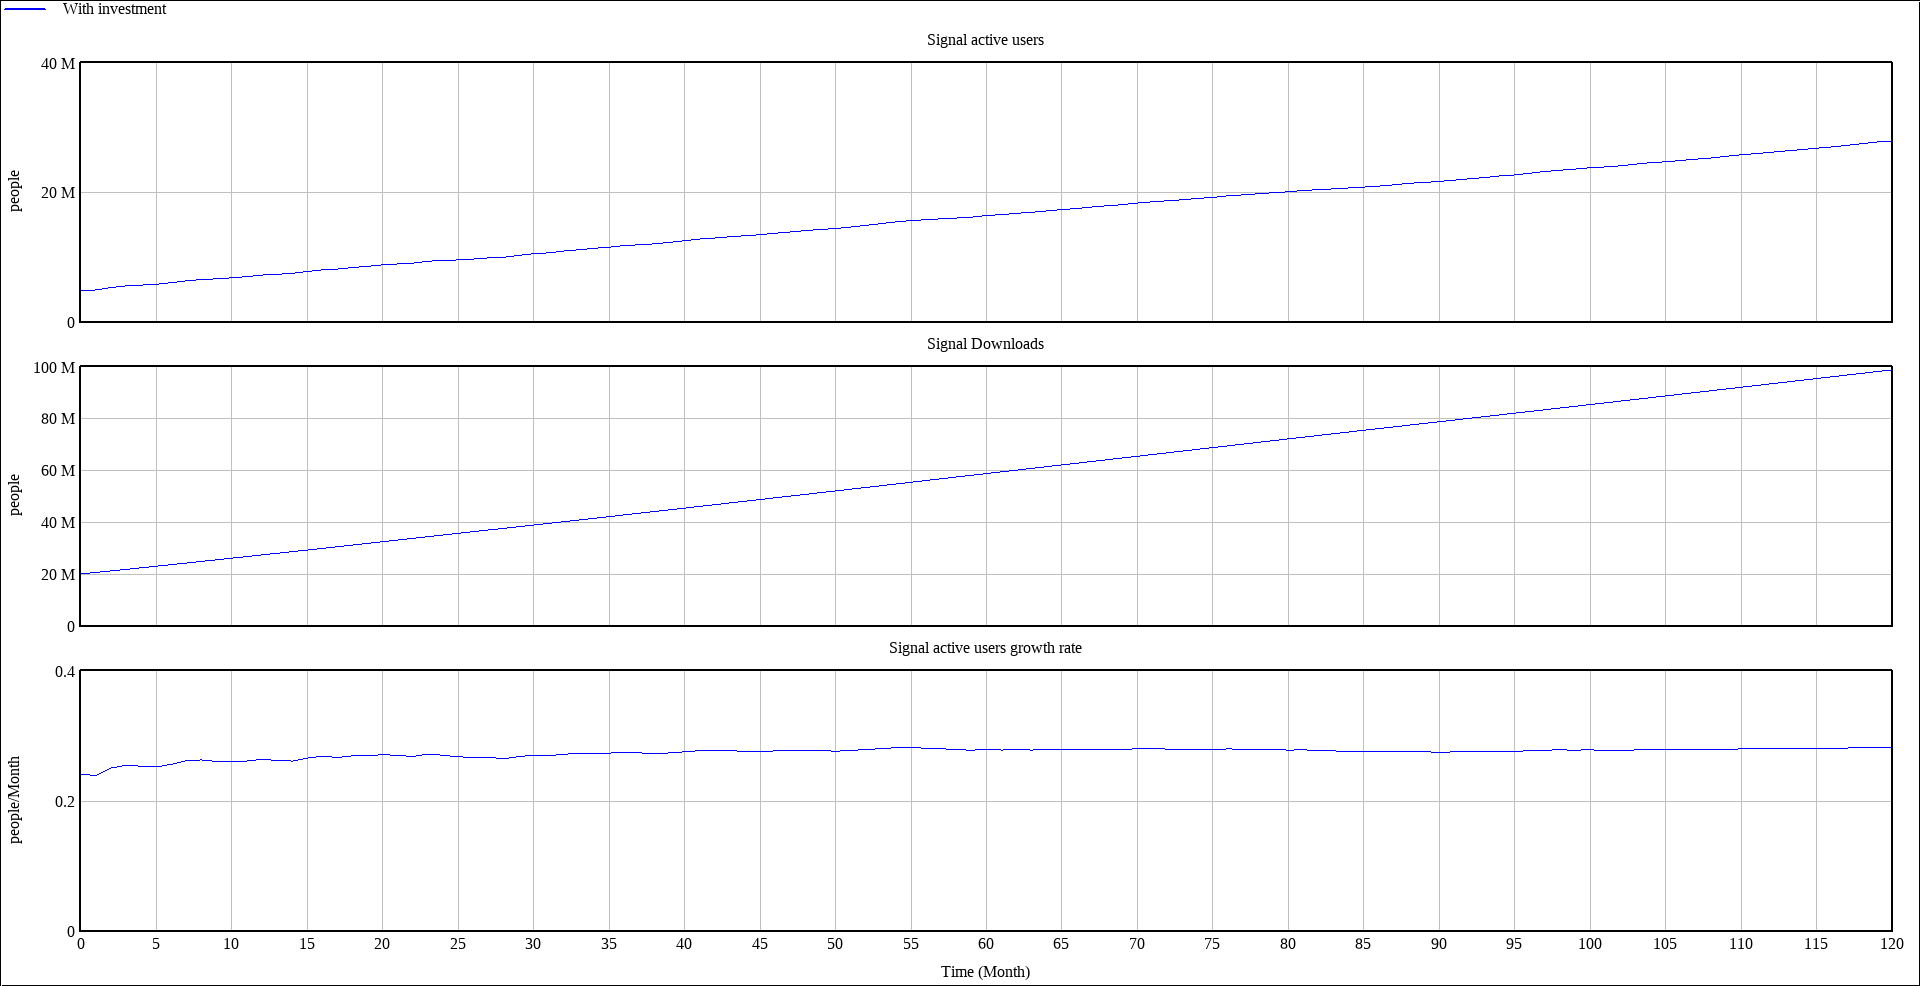
\includegraphics[width=17cm]{img/neutral_model_signal.png}
       \caption{Resultados do crescimento do número de utilizadores ativos, do número de \textit{downloads} e do valor da relação entre o número de \textit{downloads} e o número de utilizadores ativos do \textit{Signal}, obtidos numa execução neutra.}
       \label{model:base_signal_model}
   \end{center}
\end{figure}

Apesar do grande crescimento obtido, quando comparado com os dois serviços concorrentes, o número de utilizadores ativos é ainda muito inferior, como é possível verificar no gráfico da figura \ref{model:base_all_model}.

\begin{figure}[H]
   \begin{center}
       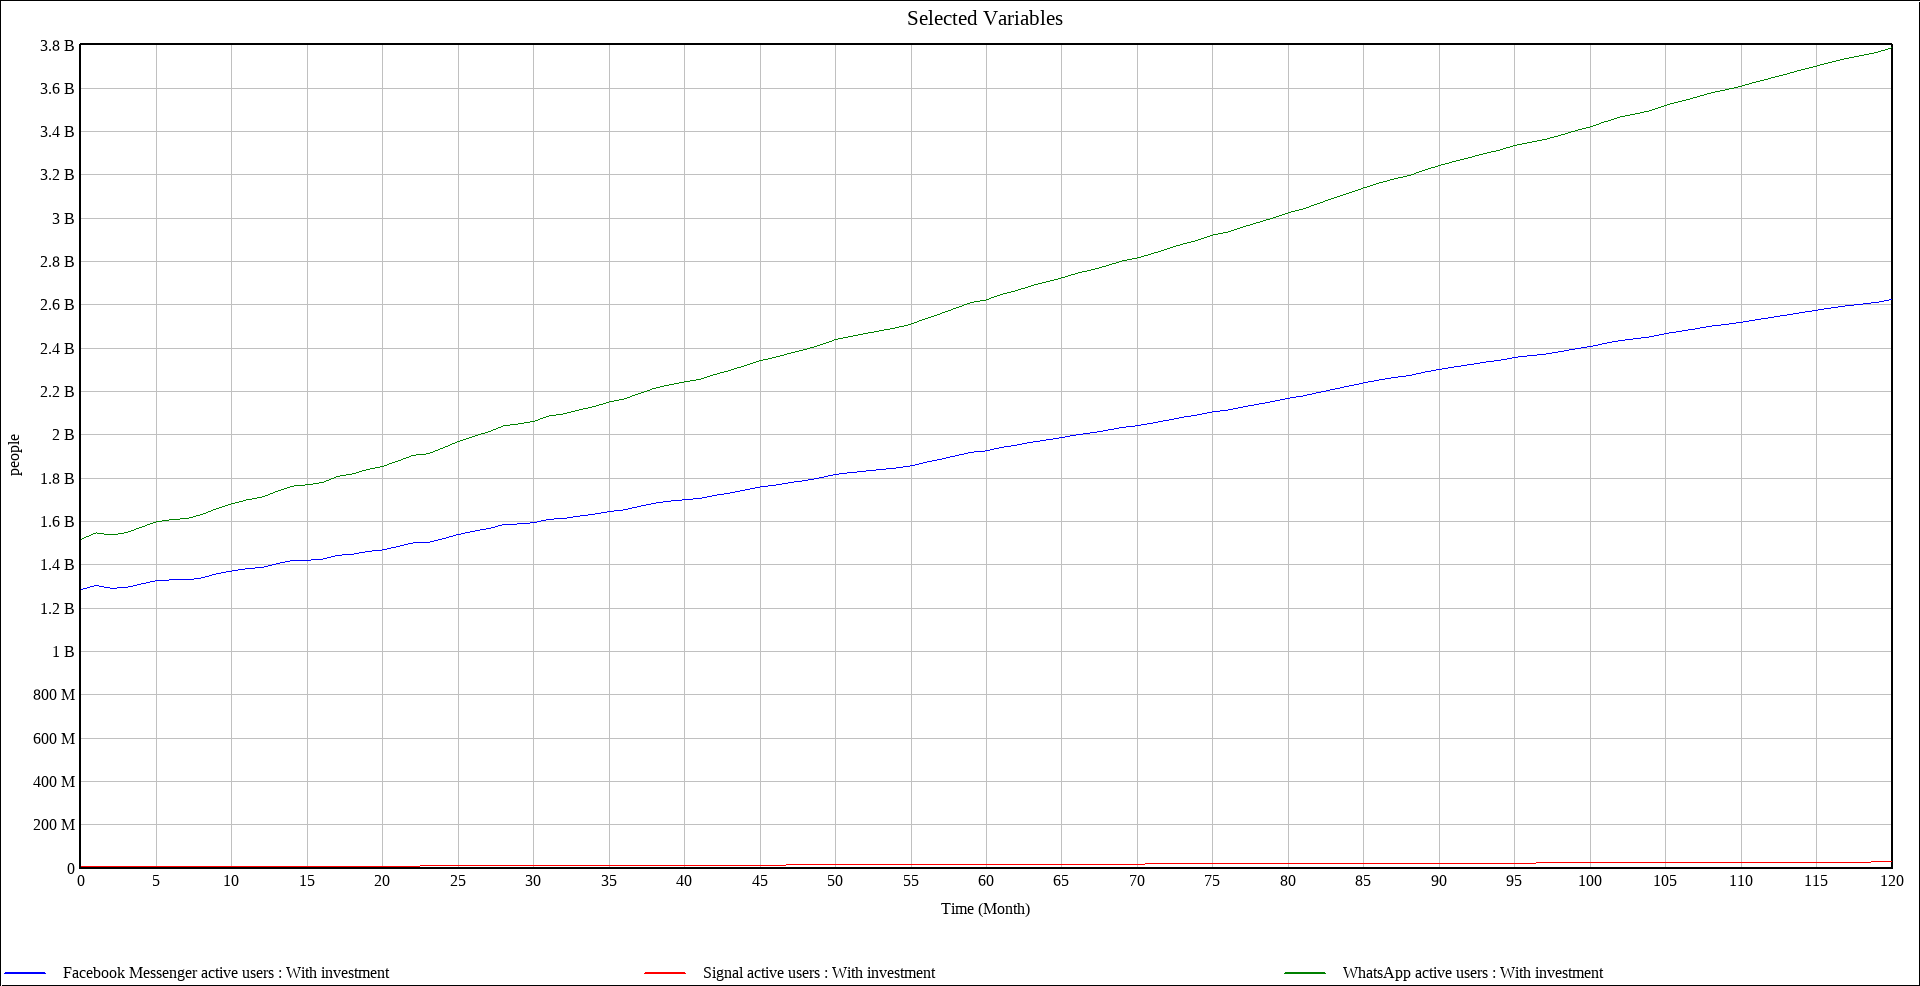
\includegraphics[width=17cm]{img/neutral_model_all.png}
       \caption{Resultados do crescimento do número de utilizadores ativos dos três serviços estudados, obtidos numa execução neutra.}
       \label{model:base_all_model}
   \end{center}
\end{figure}

Contudo, ao contrário do \textit{Signal}, as duas aplicações concorrentes tiveram uma descida ligeira ao longo do tempo no número médio de \textit{downloads} mensais, como é possível verificar na figura \ref{model:base_others_model}.

\begin{figure}[H]
   \begin{center}
       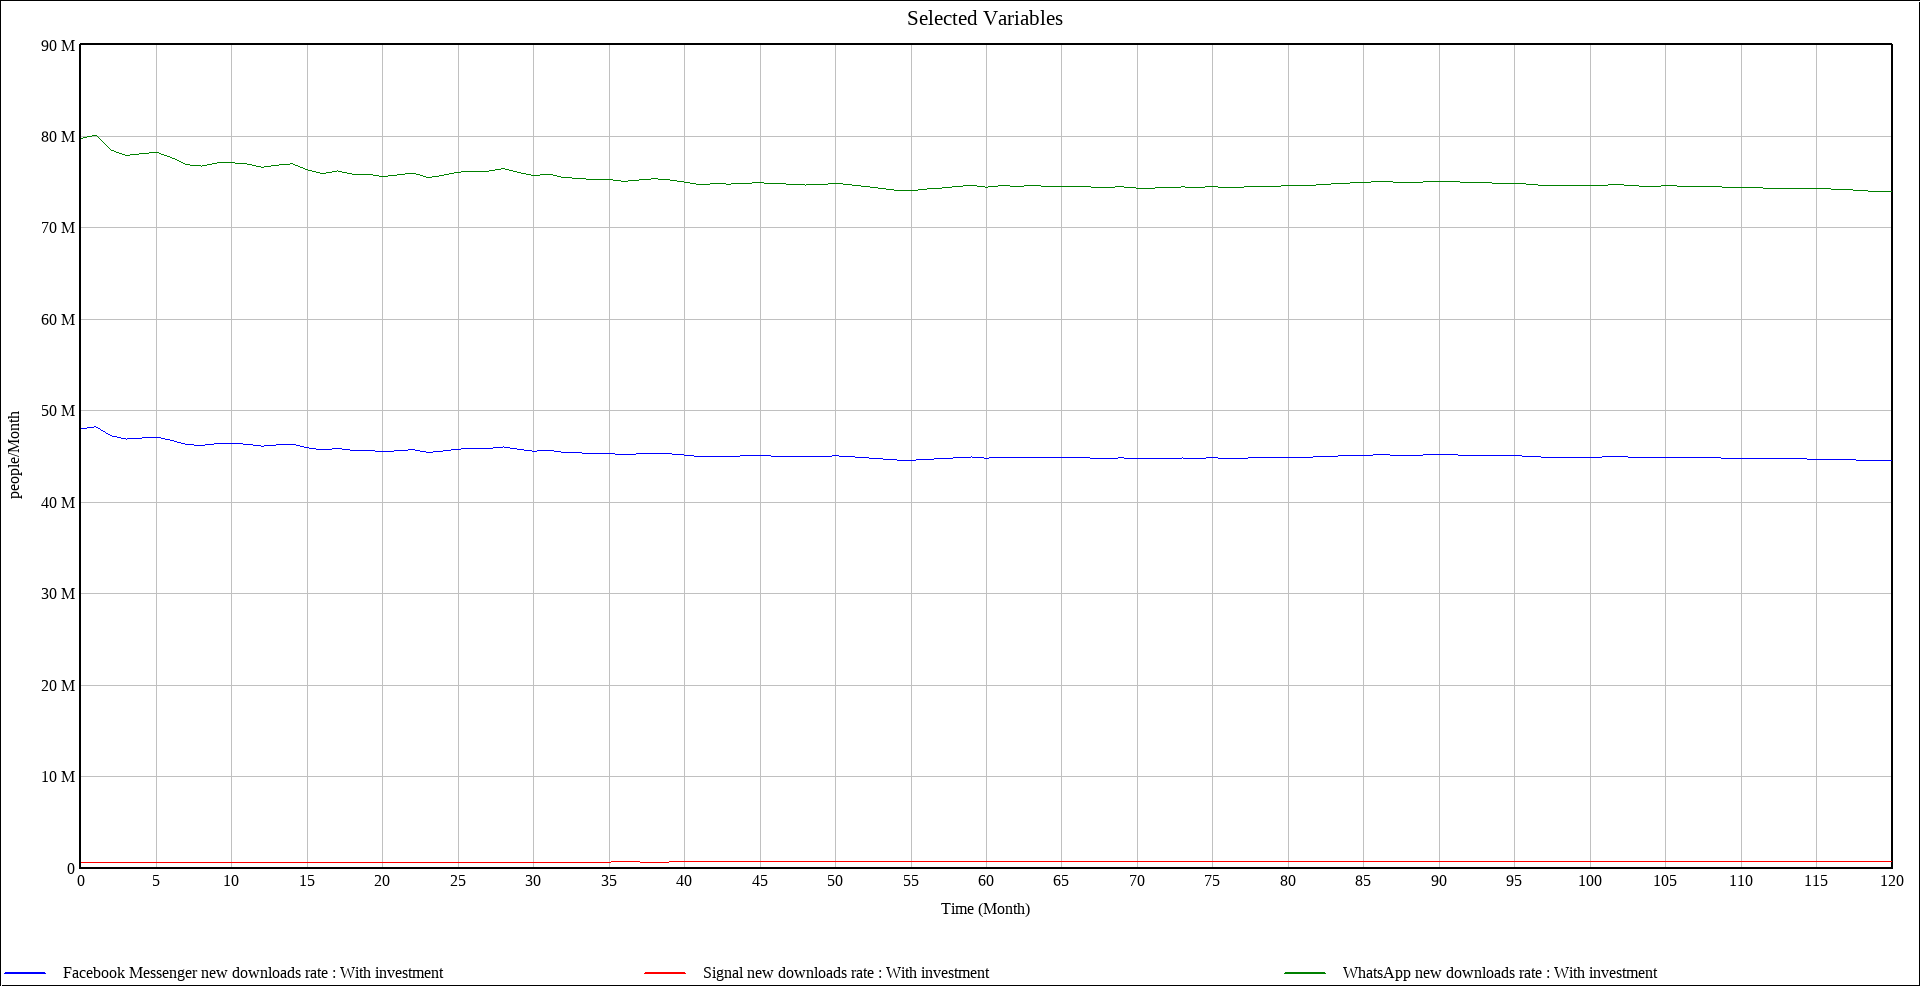
\includegraphics[width=17cm]{img/neutral_model_others_download_rate.png}
       \caption{Resultados do crescimento do número médio de \textit{downloads} mensais das aplicações concorrentes.}
       \label{model:base_others_model}
   \end{center}
\end{figure}


\subsection{Modelo pessimista}

O modelo apresentado anteriormente tem em conta que ao longo do tempo haverão investimentos de acordo com uma probabilidade hipotética. Contudo, esta probabilidade pode-se verificar muito inferior, podendo mesmo nunca chegar a haver novos investimentos. Para além disso, foi tida em conta que as aplicações concorrentes tinham um valor relativamente baixo de gastos mensais o que, dada a dimensão da empresa a que pertencem, pode não se verificar uma realidade. Desta forma, o modelo foi executado novamente, com as seguintes alterações:

\begin{itemize}
   \item Probabilidade de investimento - passou a ser $\frac{1}{100}$ ao invés de $\frac{1}{48}$.
   \item Valor máximo do investimento - passou a ser de 20 milhões ao invés de 50 milhões de dólares.
   \item Valor mínimo de investimento - passou a ser de 5 milhões ao invés de 10 milhões.
   \item Gastos mensais do \textit{WhatsApp} e \textit{Facebook Messenger}: passou a ser de 0.7 milhões ao invés de 0.4 milhões de dólares.
\end{itemize}

Nos gráficos da figura \ref{model:pessimist_signal_model} verifica-se que o caso muda de figura em relação ao modelo neutro. Apesar de se ter também um crescimento do número de utilizadores ativos do \textit{Signal}, este dá-se duma forma muito mais lenta, o número de \textit{downloads} não alcança os 80 milhões e a relação entre o número utilizadores que fazem \textit{download} da aplicação que são utilizadores ativos diminuiu lentamente, alcançando um valor inferior a 0.2 no final da simulação.

\begin{figure}[H]
   \begin{center}
       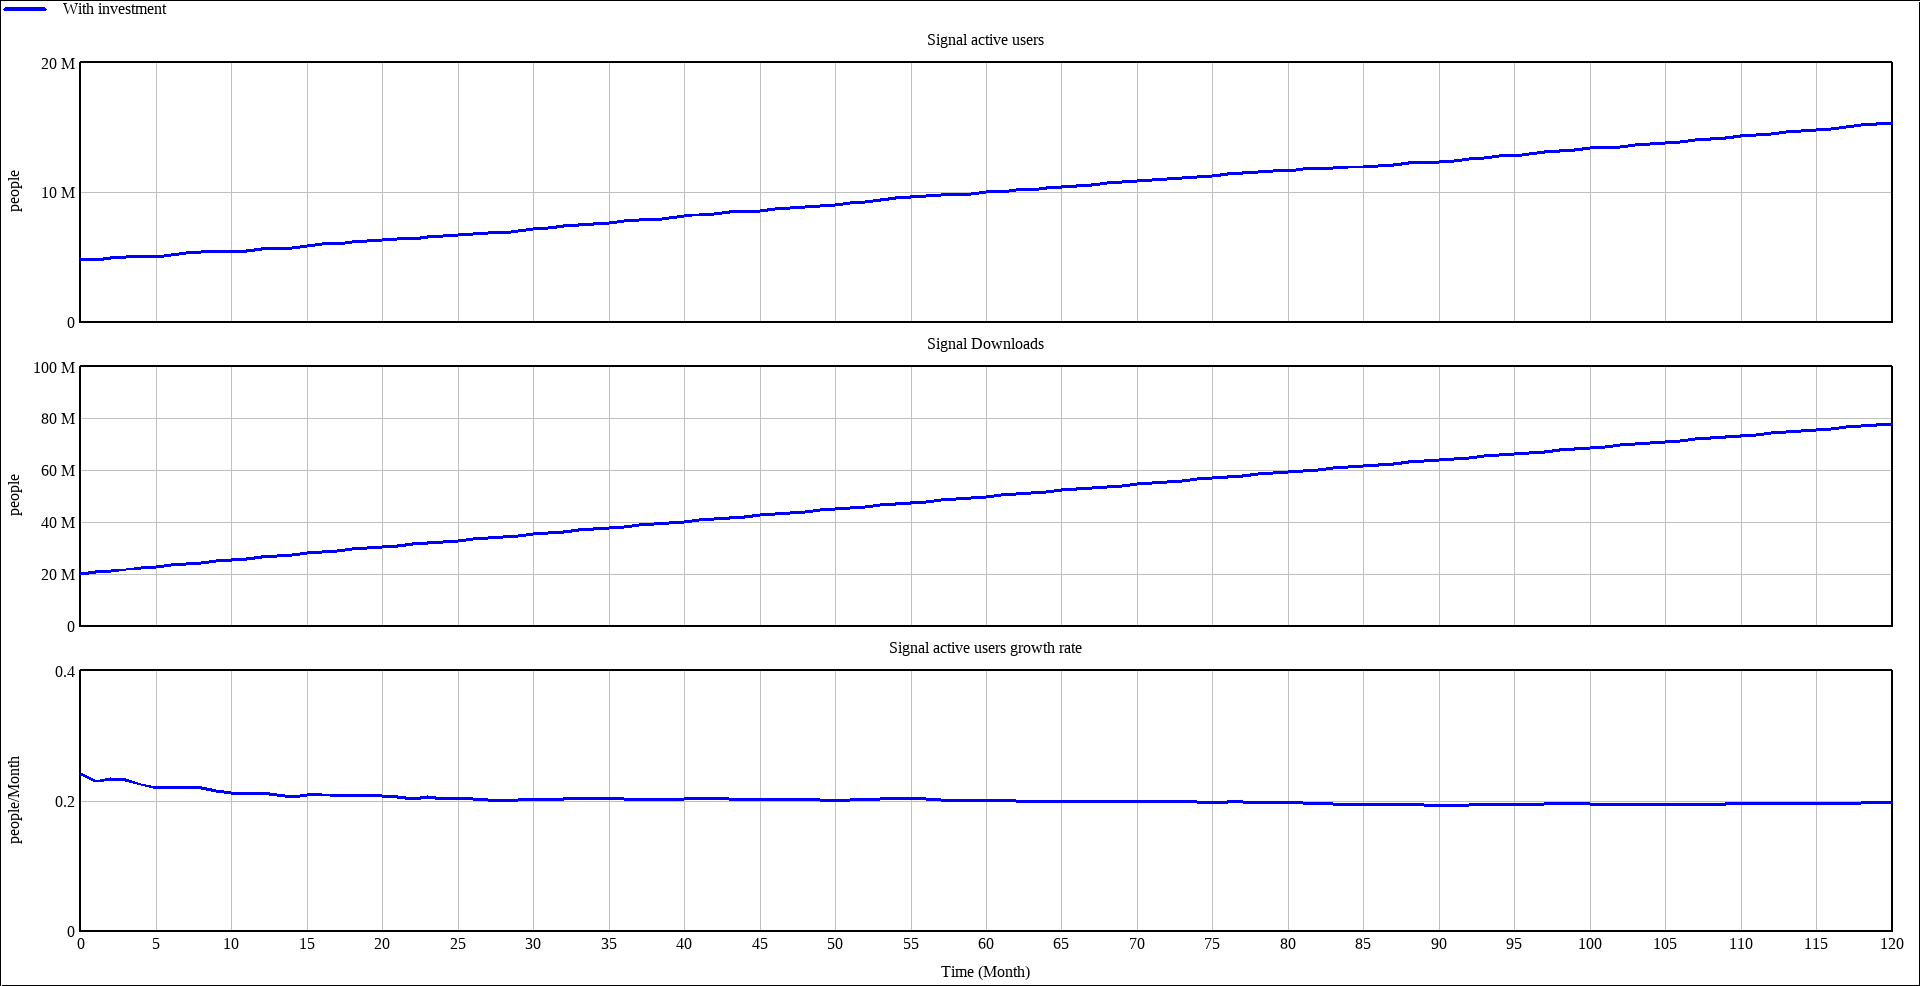
\includegraphics[width=17cm]{img/pessimist_model_signal.png}
       \caption{Resultados do crescimento do número de utilizadores ativos, do número de \textit{downloads} e do valor da relação entre o número de \textit{downloads} e o número de utilizadores ativos do \textit{Signal}, obtidos numa execução pessimista.}
       \label{model:pessimist_signal_model}
   \end{center}
\end{figure}

Como seria expectável, as duas aplicações concorrentes apresentaram um crescimento muito superior ao do modelo neutro, como se pode verificar nos gráficos da figura \ref{model:pessimist_others_model}.

\begin{figure}[H]
   \begin{center}
       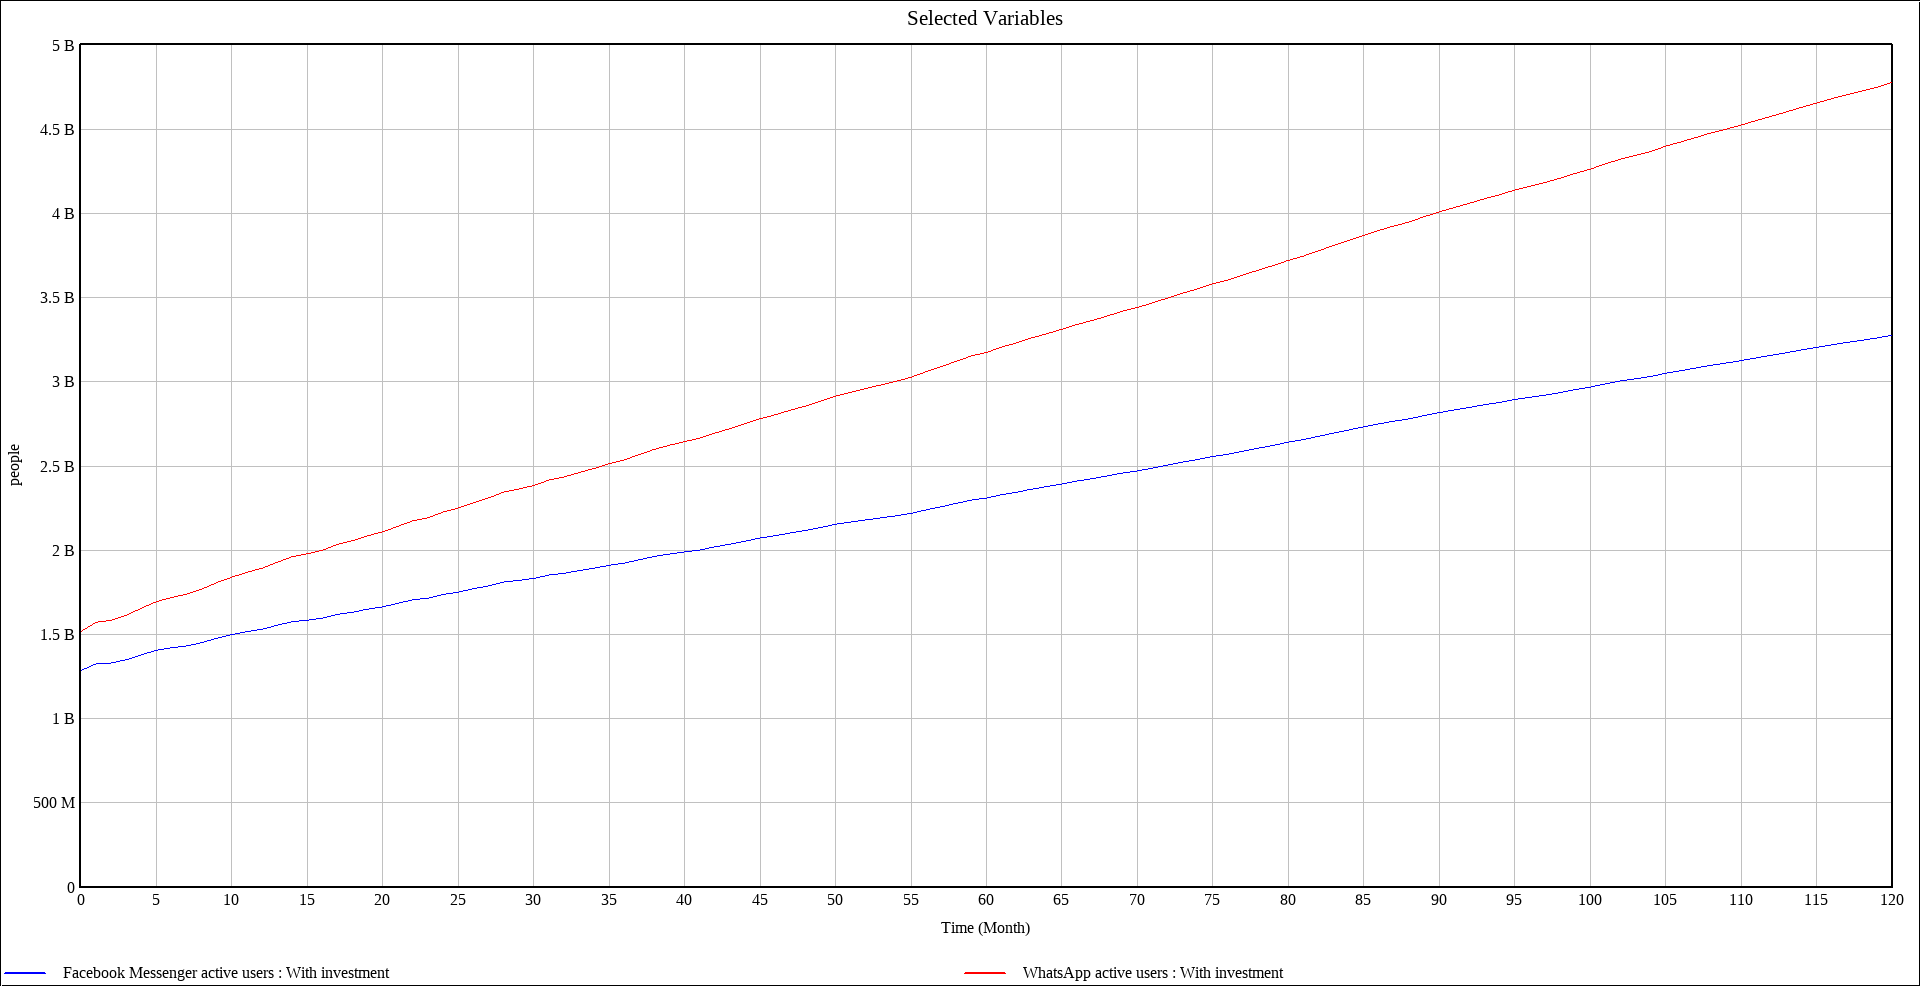
\includegraphics[width=17cm]{img/pessimist_model_others.png}
       \caption{Resultados do crescimento do número de utilizadores ativos das aplicações concorrentes, obtidos numa execução pessimista.}
       \label{model:pessimist_others_model}
   \end{center}
\end{figure}


\subsection{Modelo otimista}

Num modelo otimista foi alterada a probabilidade de ocorrerem investimentos (agora de $\frac{1}{12}$) e estes possuem agora um valor máximo superior (de 100 milhões de dólares). Para além disso, tendo em conta o maior número de investimentos, foram aumentados também os valores máximo e mínimo dos gastos mensais do \textit{Signal}, passando a ser de 1.5 e 0.7 milhões de dólares, respetivamente. Os resultados do crescimento do \textit{Signal} estão apresentados nos gráficos da figura \ref{model:optimistic_signal_model}. Como é percetível, são valores muito diferentes e superiores aos valores analisados até aqui, sendo que o número de utilizadores ativos alcança valores superiores a 40 milhões de utilizadores.

\begin{figure}[H]
   \begin{center}
       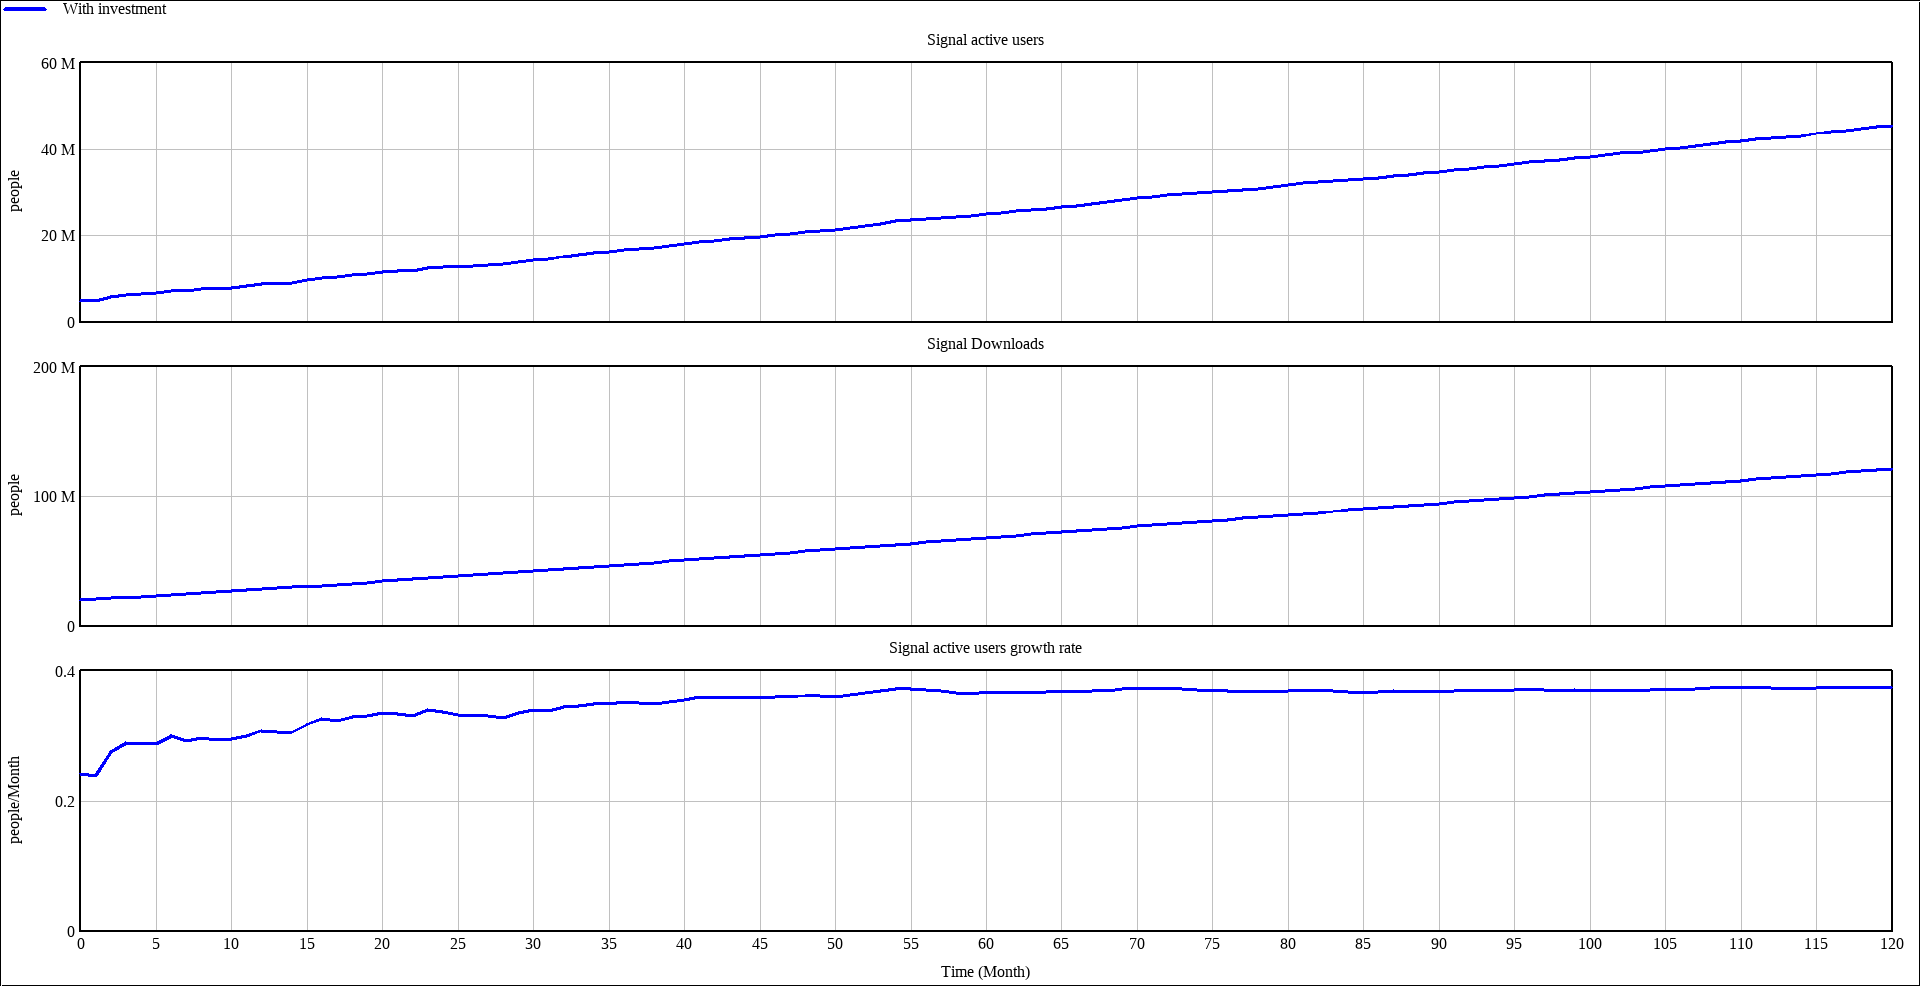
\includegraphics[width=17cm]{img/optimistic_model_signal.png}
       \caption{Resultados do crescimento do número de utilizadores ativos, do número de \textit{downloads} e do valor da relação entre o número de \textit{downloads} e o número de utilizadores ativos do \textit{Signal}, obtidos numa execução otimista.}
       \label{model:optimistic_signal_model}
   \end{center}
\end{figure}

Já as aplicações concorrentes, possuem um aumento do número de utilizadores ativos muito inferiores aos verificados nas execuções passadas, como é verificável nos gráficos da figura \ref{model:optimist_others_model}.

\begin{figure}[H]
   \begin{center}
       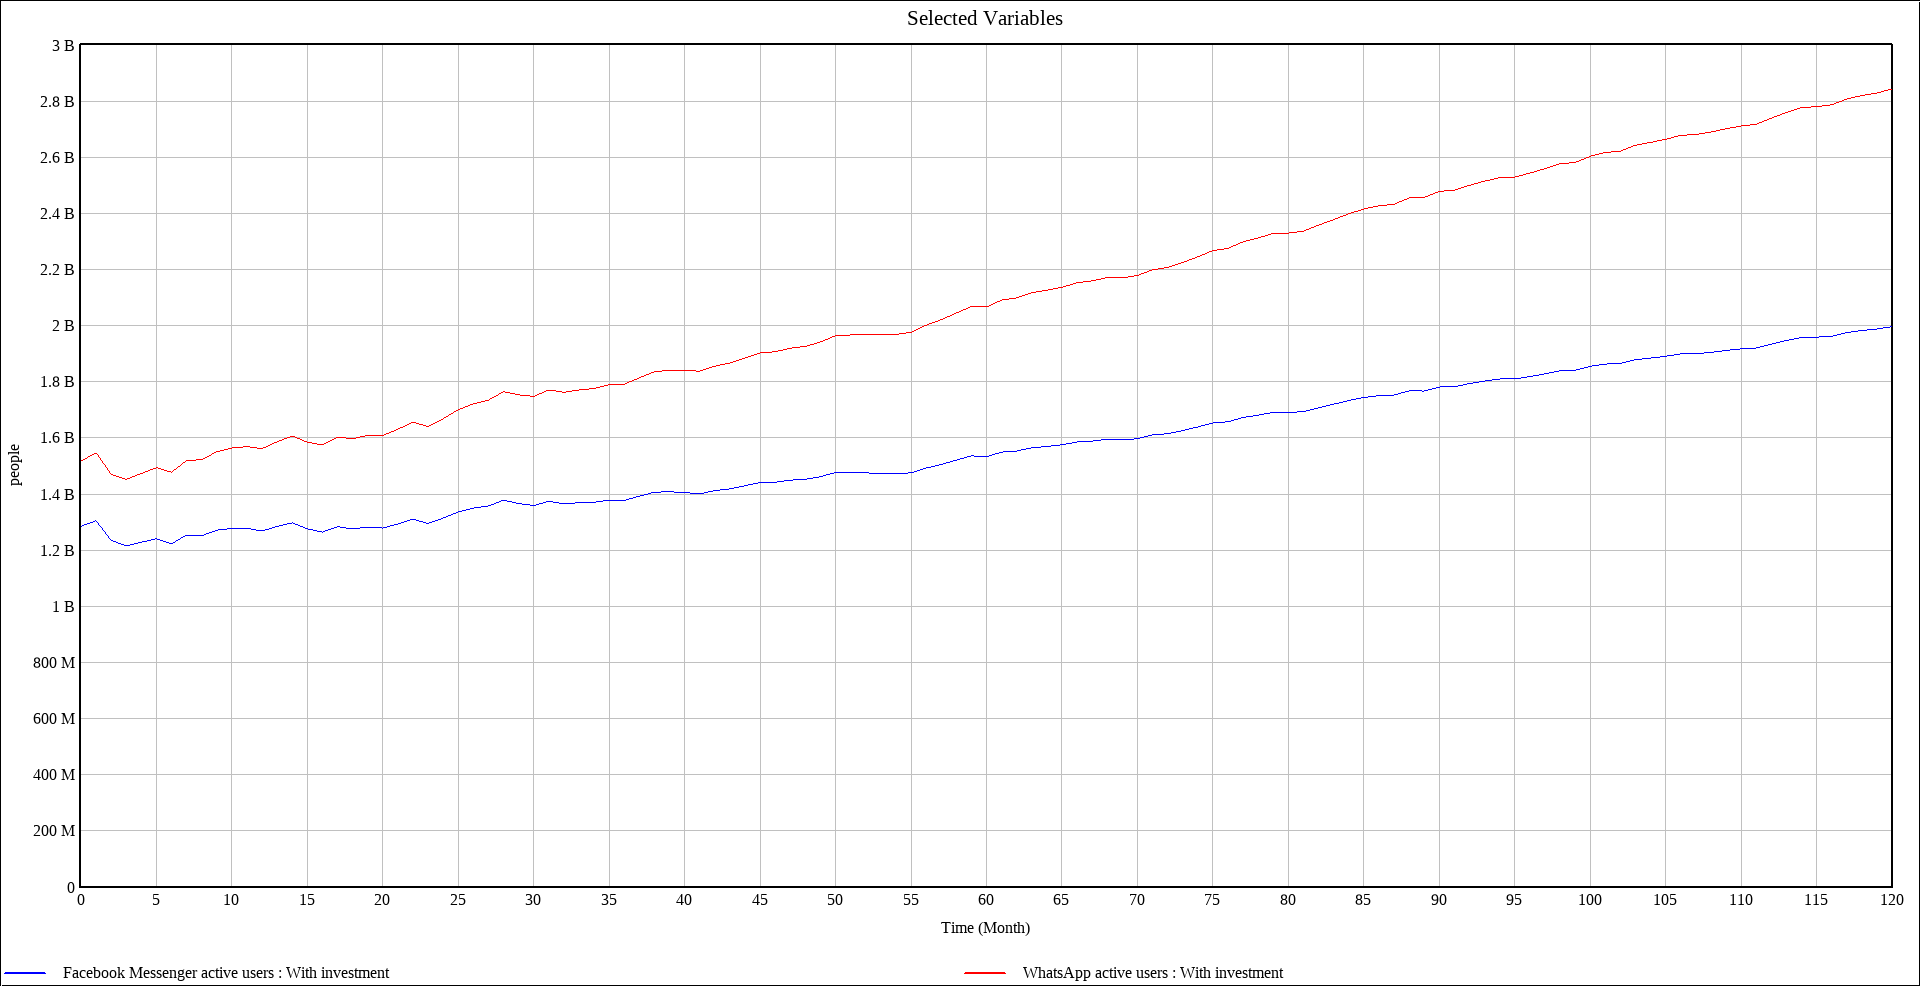
\includegraphics[width=17cm]{img/optimist_model_others.png}
       \caption{Resultados do crescimento do número de utilizadores ativos das aplicações concorrentes, obtidos numa execução otimista.}
       \label{model:optimist_others_model}
   \end{center}
\end{figure}

\section{Conclusão}

Como foi verificado nos resultados apresentados na secção \ref{sec:results}, o \textit{Signal} possivelmente terá, no futuro, um crescimento aceitável, mas lento. A não ser que se verifiquem condições similares ás apresentadas no modelo pessimista, o que é improvável, já que o co-fundador do \textit{WhatsApp} Brian Acton tem sido uma das pessoas responsáveis pelo crescimento do serviço nos últimos dois anos, sendo que algum do sucesso é devido ao mesmo \cite{wired_signal}. Contudo, a não ser que uma das aplicações concorrentes apresentadas apresente uma alteração suficientemente marcante no mercado atual, o \textit{Signal} continuará a "viver à sombra" dos serviços concorrentes.

Apesar de não se ter tido em conta no modelo apresentado, era possível ter outros fatores em conta, que poderão ser importantes no crescimento destes serviços, como por exemplo um possível aumento da consciência publica no que toca à segurança e privacidade que possuem perante entidades governamentais, entre outras possíveis fontes de crescimento.

\bibliographystyle{unsrt}
\bibliography{bibliography}

\vspace{-0.3cm}



\end{document}
